% \documentclass{standalone}
% \usepackage{currfile,hyperxmp}

% \input{../tikz_header.tex}

% \begin{document}



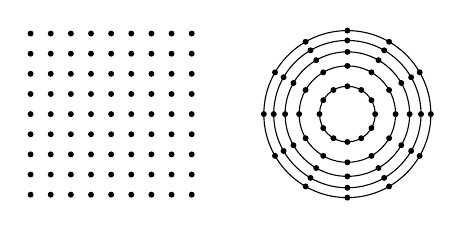
\begin{tikzpicture}
%\useasboundingbox (-1.5,-1.0) rectangle (9.1,4.2);
%\draw (-0.75,-0.75) rectangle +(1.5,1.5);

\begin{scope}

\foreach \r in {sqrt(0.5), sqrt(1.5), sqrt(2.5), sqrt(3.5), sqrt(4.5)}
 {
   \draw (0,0) circle (0.5*\r);
    \foreach \p in {0,30,...,330}
        \draw[fill=black] ({\p}:{0.5*\r}) circle (0.03);
 }

\end{scope}


\begin{scope}[xshift=-30mm]

  \foreach \i in {-4,...,4}
   {
    \foreach \j in {-4, ..., 4}
      \draw[fill=black] ({ sqrt(3.14/12) * \i *0.5}, { sqrt(3.14/12) * \j  *0.5} ) circle (0.03);
   }
  
  \end{scope}
  
  


\end{tikzpicture}

%\end{document}